\documentclass[t, aspectratio=169]{beamer}
\usepackage[utf8]{vietnam}
\usepackage{amsthm,amsmath,amssymb}
\usepackage{lmodern}
\usepackage{booktabs}
\usepackage{graphicx}
\usepackage{hyperref}

\def\slideContentLeftMargin{0.7cm}
\def\slideContentRightMargin{1cm}
\def\hustHeaderHeight{1cm}
\def\slideContentBotMargin{3.5cm}

\usepackage[blue, 169]{beamerthemeHUST}

\renewcommand{\titlePageTitleX}{-0.35cm}
\renewcommand{\titlePageTitleY}{-0.2cm}
\renewcommand{\hustTitleAlign}{\alignLeft}
\renewcommand{\hustSubtitleAlign}{\alignLeft}
\renewcommand{\hustAuthorAlign}{\alignLeft}
\renewcommand{\hustInstAlign}{\alignLeft}

\newcommand{\placeholderbox}[2]{
    \fbox{
        \begin{minipage}[c][3.6cm][c]{0.92\textwidth}
            \centering
            \textbf{#1}\\[0.4em]
            \small #2
        \end{minipage}
    }
}

\title{MULTITASK BERT FOR STUDENT SUPPORT UNDERSTANDING}
\subtitle{A self-implemented BERT encoder for SST, paraphrase detection, and STS}
\author{\texorpdfstring{Vu Thuong Tin \\ Chu Anh Duc \\ Tran Quang Hung \\ Nguyen Xuan Khai \\ Do Dang Vu}{Vu Thuong Tin, Chu Anh Duc, Tran Quang Hung, Nguyen Xuan Khai, Do Dang Vu}}
\institute{School of Information and Communication Technology -- HUST}

\begin{document}

\hustintropage{NLP Course Project}
\husttitlepage

\begin{frame}{Outline}
    \tableofcontents[hideallsubsections]
\end{frame}

\resetPageCount
\showPageNumber
\useStyleHustFull
\useThinBar

% =========================================================
\section{Problem Statement}

\begin{frame}{1. Problem Statement}
    Student-support systems often receive short natural-language requests that require different types of understanding.

    \vspace{0.5em}
    \begin{block}{Core question}
        Can one shared BERT encoder support sentiment classification, duplicate-question detection, and semantic similarity at the same time?
    \end{block}

    \vspace{0.5em}
    \begin{itemize}
        \item \textbf{Sentiment:} detect the tone of a student message.
        \item \textbf{Paraphrase:} detect duplicate or equivalent questions.
        \item \textbf{Similarity:} retrieve semantically related handbook entries.
    \end{itemize}
\end{frame}

\begin{frame}{2. Tasks and Datasets}
    \begin{center}
    \small
    \begin{tabular}{lll}
    \toprule
    Task & Dataset & Metric \\
    \midrule
    Sentiment classification & SST-5 & Accuracy \\
    Paraphrase detection & Quora Question Pairs & Accuracy \\
    Semantic similarity & STS-B & Pearson correlation \\
    \bottomrule
    \end{tabular}
    \end{center}

    \vspace{0.7em}
    The three tasks are different in output format, but all depend on contextual sentence representations.
\end{frame}

% =========================================================
\section{Approach}

\begin{frame}{3. Proposed Approach}
    \begin{columns}[T]
        \begin{column}{0.48\textwidth}
            \begin{block}{Shared representation}
                \begin{itemize}
                    \item One BERT encoder.
                    \item Three task-specific heads.
                    \item Joint multitask fine-tuning.
                \end{itemize}
            \end{block}
        \end{column}
        \begin{column}{0.48\textwidth}
            \begin{alertblock}{Main contribution}
                We re-implemented the BERT encoder ourselves instead of using \texttt{AutoModel} in the main forward path.
            \end{alertblock}
        \end{column}
    \end{columns}

    \vspace{0.6em}
    The HuggingFace backend is used only as a sanity-check reference.
\end{frame}

\begin{frame}{4. Why Multitask Learning?}
    \begin{itemize}
        \item SST learns single-sentence sentiment.
        \item Quora learns binary semantic equivalence.
        \item STS learns graded semantic similarity.
        \item Para and STS share sentence-pair structure.
    \end{itemize}

    \vspace{0.8em}
    \begin{block}{Hypothesis}
        Sharing the encoder and relational sentence-pair features can improve representation learning across related tasks.
    \end{block}
\end{frame}

% =========================================================
\section{Methodology}

\begin{frame}{5. BERT Encoder Architecture}
    \begin{columns}[T]
        \begin{column}{0.36\textwidth}
            \begin{block}{Core blocks}
                \begin{itemize}
                    \item Token ids
                    \item Token embeddings
                    \item Position embeddings
                    \item Segment embeddings
                    \item Self-attention
                    \item Feed-forward
                    \item Residual + LayerNorm
                \end{itemize}
            \end{block}
        \end{column}
        \begin{column}{0.58\textwidth}
            \begin{alertblock}{Diagram placeholder}
                \begin{itemize}
                    \item Insert BERT diagram.
                    \item Input $\rightarrow$ embeddings.
                    \item Encoder stack.
                    \item \texttt{[CLS]} output.
                \end{itemize}
            \end{alertblock}
        \end{column}
    \end{columns}
\end{frame}

\begin{frame}{6. Self-Implementation Validation}
    \begin{block}{Parity check against HuggingFace}
        Same input and same pretrained weights:
        \begin{itemize}
            \item Max hidden-state difference: $4.29\times10^{-6}$.
            \item Max pooler-output difference: $9.54\times10^{-7}$.
        \end{itemize}
    \end{block}

    \vspace{0.6em}
    This validates that the custom encoder is numerically faithful before fine-tuning.
\end{frame}

\begin{frame}{7. Multitask Architecture}
    \begin{center}
    \small
    \begin{tabular}{lll}
    \toprule
    Component & Role & Output \\
    \midrule
    Shared BERT encoder & Contextual representation & \texttt{[CLS]} vector \\
    SST head & Sentiment classifier & 5 logits \\
    Paraphrase head & Duplicate detector & 1 logit \\
    STS head & Similarity regressor & score in $[0,5]$ \\
    Relational layer & Shared Para--STS features & pair interaction \\
    \bottomrule
    \end{tabular}
    \end{center}

    \vspace{0.5em}
    The architecture separates task-specific decisions while keeping the language representation shared.
\end{frame}

\begin{frame}{8. Rich Relational Layer}
    Para and STS are both sentence-pair tasks. We therefore share an interaction representation before branching into task-specific heads.

    \[
        z = \frac{h_u \odot h_v}{\|h_u\|_2\|h_v\|_2+\epsilon}
    \]

    \begin{itemize}
        \item $h_u, h_v$: pooled sentence vectors.
        \item Element-wise interaction keeps dimension-level information.
        \item STS can benefit from the larger Quora signal.
    \end{itemize}
\end{frame}

% =========================================================
\section{Training}

\begin{frame}{9. Training Pipeline}
    \begin{columns}[T]
        \begin{column}{0.44\textwidth}
            \begin{block}{Pipeline}
                \begin{itemize}
                    \item Load tokenizer
                    \item Load BERT weights
                    \item Build dataloaders
                    \item Interleaved batches
                    \item Task losses
                    \item Save best checkpoint
                \end{itemize}
            \end{block}
        \end{column}
        \begin{column}{0.50\textwidth}
            \begin{alertblock}{Diagram placeholder}
                \begin{itemize}
                    \item Insert training flow.
                    \item SST / Para / STS.
                    \item Shared encoder.
                    \item Task heads.
                    \item Aggregate score.
                \end{itemize}
            \end{alertblock}
        \end{column}
    \end{columns}
\end{frame}

\begin{frame}{10. Optimization Setup}
    \begin{block}{Best recipe}
        \begin{itemize}
            \item Optimizer: AdamW.
            \item Learning rate: $2e^{-5}$.
            \item Weight decay: 0.01.
            \item Epochs: 20.
            \item Schedule: linear warmup/decay.
        \end{itemize}
    \end{block}

    \vspace{0.5em}
    Checkpoints are selected by aggregate development score.
\end{frame}

% =========================================================
\section{Results}

\begin{frame}{11. Evaluation Protocol}
    Each task is evaluated with its standard metric:

    \begin{itemize}
        \item SST: accuracy.
        \item Paraphrase: accuracy.
        \item STS: Pearson correlation.
    \end{itemize}

    \vspace{0.5em}
    Aggregate score:
    \[
        S = \frac{\text{SST}_{acc} + \text{Para}_{acc} + (\text{STS}_{r}+1)/2}{3}
    \]
\end{frame}

\begin{frame}{12. Main Results}
    \begin{center}
    \small
    \begin{tabular}{lcccc}
    \toprule
    Model & SST & Para & STS & Score \\
    \midrule
    Self-impl AdamW linear 20e & 0.520 & \textbf{0.864} & 0.785 & \textbf{0.759} \\
    HF sanity baseline 10e & \textbf{0.526} & 0.861 & \textbf{0.790} & 0.761 \\
    Self-impl AdamW constant LR & 0.505 & 0.860 & 0.784 & 0.752 \\
    Self-impl Muon safe 20e & 0.523 & 0.851 & 0.750 & 0.750 \\
    Muon high-LR early run & 0.262 & 0.720 & 0.145 & 0.518 \\
    \bottomrule
    \end{tabular}
    \end{center}

    \vspace{0.4em}
    Our self-implemented encoder reaches 0.759, nearly matching the library-backed baseline at 0.761.
\end{frame}

\begin{frame}{13. Optimizer Finding}
    \begin{columns}[T]
        \begin{column}{0.56\textwidth}
            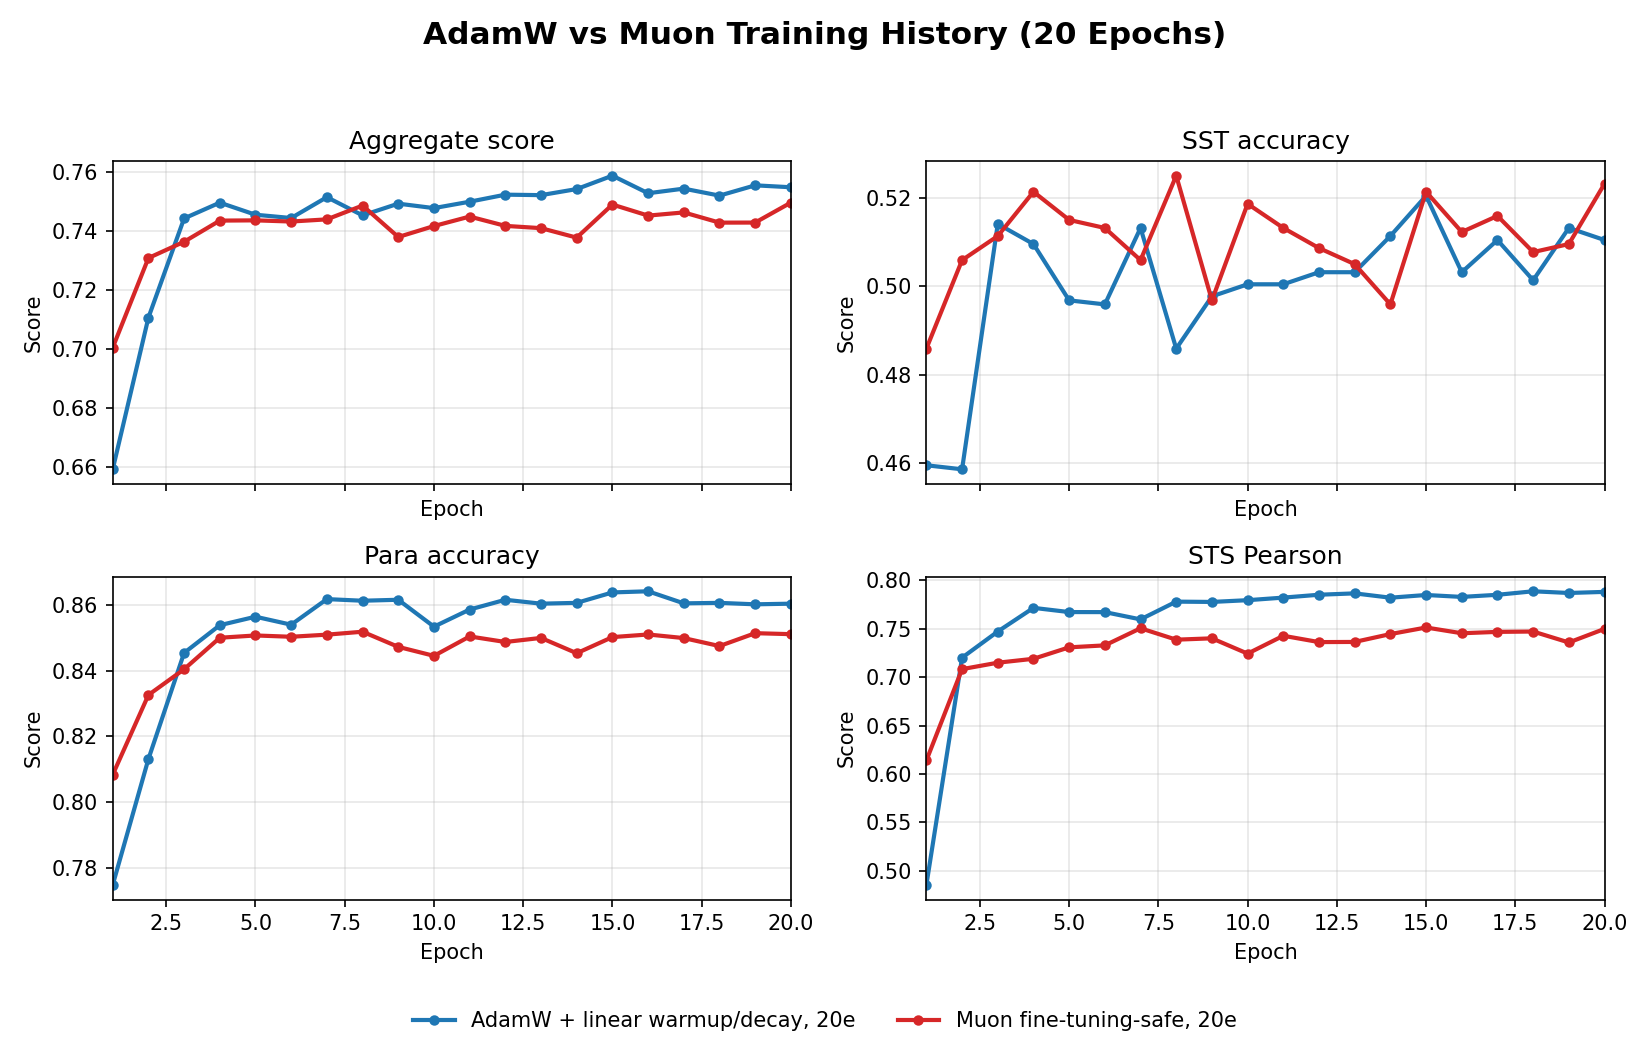
\includegraphics[width=\textwidth]{adamw_vs_muon_history.png}
        \end{column}
        \begin{column}{0.40\textwidth}
            \begin{block}{Conclusion}
                \begin{itemize}
                    \item AdamW is clearly better.
                    \item Muon damages pretrained weights.
                    \item Para / STS drop sharply.
                    \item Final choice: AdamW.
                \end{itemize}
            \end{block}
        \end{column}
    \end{columns}
\end{frame}

\begin{frame}{14. Error Analysis}
    \begin{block}{Current weakness}
        STS is the weakest task: Pearson $r=0.785$.
    \end{block}

    \vspace{0.5em}
    \begin{alertblock}{To complete}
        Insert 2--3 real STS error examples:
        \begin{itemize}
            \item sentence A / sentence B,
            \item gold score / predicted score,
            \item short error explanation.
        \end{itemize}
    \end{alertblock}
\end{frame}

% =========================================================
\section{Demo}

\begin{frame}{15. Demo A: Checkpoint Inference}
    \begin{columns}[T]
        \begin{column}{0.48\textwidth}
            \begin{block}{Purpose}
                Directly load one checkpoint and test:
                \begin{itemize}
                    \item SST sentiment.
                    \item Paraphrase probability.
                    \item STS similarity score.
                \end{itemize}
            \end{block}
            \small \texttt{scripts/demo\_gradio.py}
        \end{column}
        \begin{column}{0.48\textwidth}
            \placeholderbox{Screenshot Placeholder}{Replace with checkpoint inference screenshot.}
        \end{column}
    \end{columns}
\end{frame}

\begin{frame}{16. Demo B: Smart Student Support}
    \begin{columns}[T]
        \begin{column}{0.48\textwidth}
            \begin{block}{Product workflow}
                \begin{itemize}
                    \item Detect student sentiment.
                    \item Match duplicate FAQs.
                    \item Rank handbook entries.
                \end{itemize}
            \end{block}
            \small \texttt{scripts/demo\_student\_support.py}
        \end{column}
        \begin{column}{0.48\textwidth}
            \placeholderbox{Screenshot Placeholder}{Replace with Smart Student Support screenshot.}
        \end{column}
    \end{columns}
\end{frame}

\begin{frame}{17. Demo Commands}
    \small
    \begin{block}{Checkpoint inference}
    \texttt{PYTHONPATH=src python -m scripts.demo\_gradio \textbackslash}\\
    \texttt{\quad --config configs/report\_best\_self\_impl\_20e\_linear\_warmup\_lr2e5.yaml \textbackslash}\\
    \texttt{\quad --checkpoint runs/report\_best\_self\_impl\_20e\_linear\_warmup\_lr2e5/best.pt}
    \end{block}

    \begin{block}{Smart student support}
    \texttt{PYTHONPATH=src python -m scripts.demo\_student\_support \textbackslash}\\
    \texttt{\quad --config configs/report\_best\_self\_impl\_20e\_linear\_warmup\_lr2e5.yaml \textbackslash}\\
    \texttt{\quad --checkpoint runs/report\_best\_self\_impl\_20e\_linear\_warmup\_lr2e5/best.pt}
    \end{block}
\end{frame}

% =========================================================
\section{Conclusions}

\begin{frame}{18. Conclusions}
    \begin{itemize}
        \item We re-implemented the BERT encoder.
        \item Encoder parity is extremely close: $4.29\times10^{-6}$.
        \item Self-implemented score: \textbf{0.759}.
        \item HF baseline score: 0.761.
        \item AdamW clearly outperforms Muon.
        \item Two demos connect benchmarks to usage.
    \end{itemize}

    \vspace{0.5em}
    Future work: stronger STS calibration, dynamic task weighting, and richer sentence-pair modeling.
\end{frame}

\hustcontactpage{\hfill THANK YOU \hfill}{
    \textbf{Project:} Multitask BERT for Student Support Understanding \\
    \textbf{Repository:} \texttt{multitask-bert-v2} \\
    \vspace{0.5cm}
    \textit{Q\&A}
}

\useStyleLogoOnly
\setbeamertemplate{bibliography item}[text]

\begin{frame}{References}
    \begin{thebibliography}{9}
        \bibitem{bert} Devlin et al., \emph{BERT: Pre-training of Deep Bidirectional Transformers for Language Understanding}, 2019.
        \bibitem{mtdnn} Liu et al., \emph{Multi-Task Deep Neural Networks for Natural Language Understanding}, 2019.
        \bibitem{sbert} Reimers and Gurevych, \emph{Sentence-BERT}, 2019.
        \bibitem{adamw} Loshchilov and Hutter, \emph{Decoupled Weight Decay Regularization}, 2019.
    \end{thebibliography}
\end{frame}

\end{document}
